\documentclass[a4paper, 12pt]{article}

% ~~~~~~~~~~~~~~~~~~~~~~~~~~~~~~~~~~~~~~~~
% ~~~~~~~~~~~~~~~ PACKAGES ~~~~~~~~~~~~~~~
% ~~~~~~~~~~~~~~~~~~~~~~~~~~~~~~~~~~~~~~~~

\usepackage{relsize}
\usepackage{tikz}
\usetikzlibrary{positioning}
\usetikzlibrary{arrows}

% ~~~~~~~~~~~~~~~~~~~~~~~~~~~~~~~~~~~~~~~~
% ~~~~~~~~~~~~~~~ PREAMBLE ~~~~~~~~~~~~~~~
% ~~~~~~~~~~~~~~~~~~~~~~~~~~~~~~~~~~~~~~~~

\title{Demo Document No. 2\\[0.4em]\smaller{for the SEPTeX module}}
\author{Marcel Simader}
\date{}
\pagenumbering{gobble}

% ~~~~~~~~~~~~~~~~~~~~~~~~~~~~~~~~~~~~
% ~~~~~~~~~~~~~~~ BODY ~~~~~~~~~~~~~~~
% ~~~~~~~~~~~~~~~~~~~~~~~~~~~~~~~~~~~~

\begin{document}
	\maketitle
	
	\begin{center}
		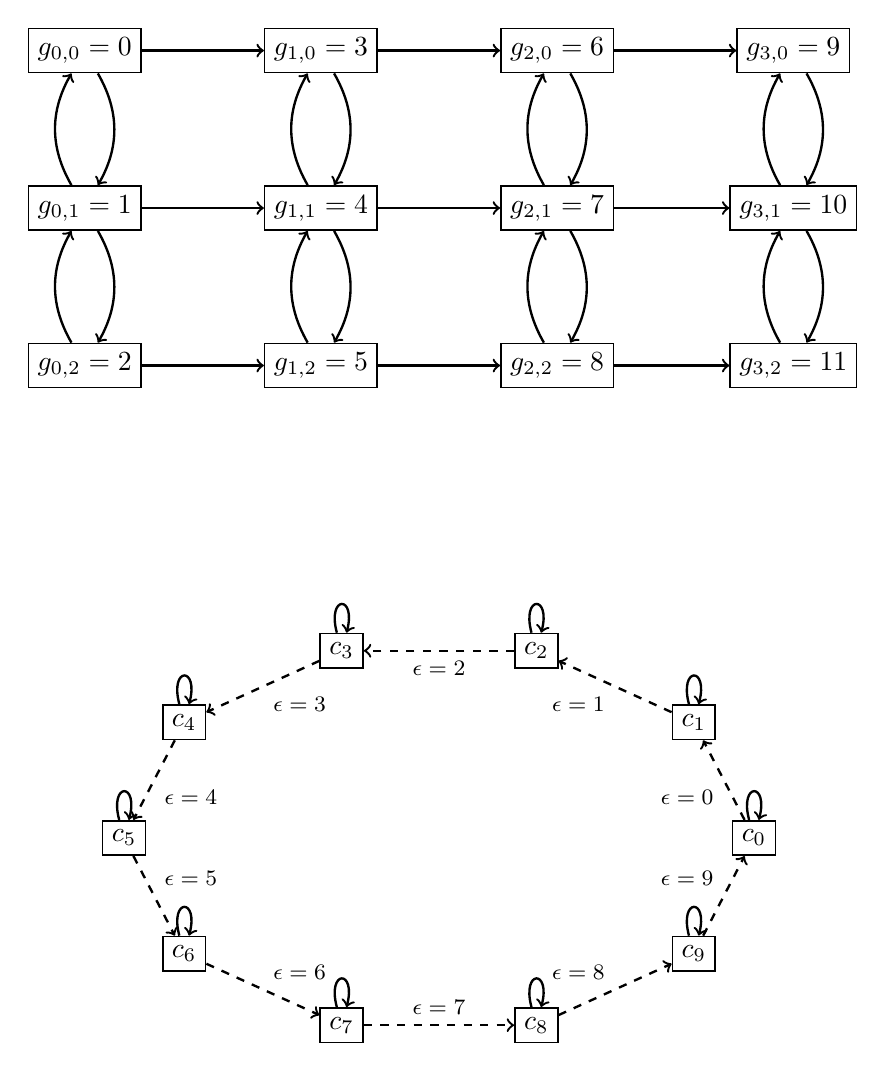
\begin{tikzpicture}[draw]
			\node[draw, line width={0.2mm}] (grid-0-0) at ( 0.0000000,  0.0000000) {$g_{0,0}=0$};
			\node[draw, line width={0.2mm}] (grid-0-1) at ( 0.0000000, -2.0000000) {$g_{0,1}=1$};
			\node[draw, line width={0.2mm}] (grid-0-2) at ( 0.0000000, -4.0000000) {$g_{0,2}=2$};
			\node[draw, line width={0.2mm}] (grid-1-0) at ( 3.0000000,  0.0000000) {$g_{1,0}=3$};
			\node[draw, line width={0.2mm}] (grid-1-1) at ( 3.0000000, -2.0000000) {$g_{1,1}=4$};
			\node[draw, line width={0.2mm}] (grid-1-2) at ( 3.0000000, -4.0000000) {$g_{1,2}=5$};
			\node[draw, line width={0.2mm}] (grid-2-0) at ( 6.0000000,  0.0000000) {$g_{2,0}=6$};
			\node[draw, line width={0.2mm}] (grid-2-1) at ( 6.0000000, -2.0000000) {$g_{2,1}=7$};
			\node[draw, line width={0.2mm}] (grid-2-2) at ( 6.0000000, -4.0000000) {$g_{2,2}=8$};
			\node[draw, line width={0.2mm}] (grid-3-0) at ( 9.0000000,  0.0000000) {$g_{3,0}=9$};
			\node[draw, line width={0.2mm}] (grid-3-1) at ( 9.0000000, -2.0000000) {$g_{3,1}=10$};
			\node[draw, line width={0.2mm}] (grid-3-2) at ( 9.0000000, -4.0000000) {$g_{3,2}=11$};
			\node[draw, line width={0.2mm}] (circ-0) at ( 8.5000000, -10.0000000) {$c_{0}$};
			\node[draw, line width={0.2mm}] (circ-1) at ( 7.7360680, -8.5305369) {$c_{1}$};
			\node[draw, line width={0.2mm}] (circ-2) at ( 5.7360680, -7.6223587) {$c_{2}$};
			\node[draw, line width={0.2mm}] (circ-3) at ( 3.2639320, -7.6223587) {$c_{3}$};
			\node[draw, line width={0.2mm}] (circ-4) at ( 1.2639320, -8.5305369) {$c_{4}$};
			\node[draw, line width={0.2mm}] (circ-5) at ( 0.5000000, -10.0000000) {$c_{5}$};
			\node[draw, line width={0.2mm}] (circ-6) at ( 1.2639320, -11.4694631) {$c_{6}$};
			\node[draw, line width={0.2mm}] (circ-7) at ( 3.2639320, -12.3776413) {$c_{7}$};
			\node[draw, line width={0.2mm}] (circ-8) at ( 5.7360680, -12.3776413) {$c_{8}$};
			\node[draw, line width={0.2mm}] (circ-9) at ( 7.7360680, -11.4694631) {$c_{9}$};
			\draw[->, draw, line width={0.3mm}] (grid-0-0) to (grid-1-0);
			\draw[->, bend left, draw, line width={0.3mm}] (grid-0-0) to (grid-0-1);
			\draw[<-, bend right, draw, line width={0.3mm}] (grid-0-0) to (grid-0-1);
			\draw[->, draw, line width={0.3mm}] (grid-1-0) to (grid-2-0);
			\draw[->, bend left, draw, line width={0.3mm}] (grid-1-0) to (grid-1-1);
			\draw[<-, bend right, draw, line width={0.3mm}] (grid-1-0) to (grid-1-1);
			\draw[->, draw, line width={0.3mm}] (grid-2-0) to (grid-3-0);
			\draw[->, bend left, draw, line width={0.3mm}] (grid-2-0) to (grid-2-1);
			\draw[<-, bend right, draw, line width={0.3mm}] (grid-2-0) to (grid-2-1);
			\draw[->, bend left, draw, line width={0.3mm}] (grid-3-0) to (grid-3-1);
			\draw[<-, bend right, draw, line width={0.3mm}] (grid-3-0) to (grid-3-1);
			\draw[->, draw, line width={0.3mm}] (grid-0-1) to (grid-1-1);
			\draw[->, bend left, draw, line width={0.3mm}] (grid-0-1) to (grid-0-2);
			\draw[<-, bend right, draw, line width={0.3mm}] (grid-0-1) to (grid-0-2);
			\draw[->, draw, line width={0.3mm}] (grid-1-1) to (grid-2-1);
			\draw[->, bend left, draw, line width={0.3mm}] (grid-1-1) to (grid-1-2);
			\draw[<-, bend right, draw, line width={0.3mm}] (grid-1-1) to (grid-1-2);
			\draw[->, draw, line width={0.3mm}] (grid-2-1) to (grid-3-1);
			\draw[->, bend left, draw, line width={0.3mm}] (grid-2-1) to (grid-2-2);
			\draw[<-, bend right, draw, line width={0.3mm}] (grid-2-1) to (grid-2-2);
			\draw[->, bend left, draw, line width={0.3mm}] (grid-3-1) to (grid-3-2);
			\draw[<-, bend right, draw, line width={0.3mm}] (grid-3-1) to (grid-3-2);
			\draw[->, draw, line width={0.3mm}] (grid-0-2) to (grid-1-2);
			\draw[->, draw, line width={0.3mm}] (grid-1-2) to (grid-2-2);
			\draw[->, draw, line width={0.3mm}] (grid-2-2) to (grid-3-2);
			\draw[->, draw, dashed, line width={0.3mm}] (circ-0) to node [auto] {\footnotesize$\epsilon=0$} (circ-1);
			\draw[->, loop above, draw, line width={0.3mm}] (circ-0) to (circ-0);
			\draw[->, draw, dashed, line width={0.3mm}] (circ-1) to node [auto] {\footnotesize$\epsilon=1$} (circ-2);
			\draw[->, loop above, draw, line width={0.3mm}] (circ-1) to (circ-1);
			\draw[->, draw, dashed, line width={0.3mm}] (circ-2) to node [auto] {\footnotesize$\epsilon=2$} (circ-3);
			\draw[->, loop above, draw, line width={0.3mm}] (circ-2) to (circ-2);
			\draw[->, draw, dashed, line width={0.3mm}] (circ-3) to node [auto] {\footnotesize$\epsilon=3$} (circ-4);
			\draw[->, loop above, draw, line width={0.3mm}] (circ-3) to (circ-3);
			\draw[->, draw, dashed, line width={0.3mm}] (circ-4) to node [auto] {\footnotesize$\epsilon=4$} (circ-5);
			\draw[->, loop above, draw, line width={0.3mm}] (circ-4) to (circ-4);
			\draw[->, draw, dashed, line width={0.3mm}] (circ-5) to node [auto] {\footnotesize$\epsilon=5$} (circ-6);
			\draw[->, loop above, draw, line width={0.3mm}] (circ-5) to (circ-5);
			\draw[->, draw, dashed, line width={0.3mm}] (circ-6) to node [auto] {\footnotesize$\epsilon=6$} (circ-7);
			\draw[->, loop above, draw, line width={0.3mm}] (circ-6) to (circ-6);
			\draw[->, draw, dashed, line width={0.3mm}] (circ-7) to node [auto] {\footnotesize$\epsilon=7$} (circ-8);
			\draw[->, loop above, draw, line width={0.3mm}] (circ-7) to (circ-7);
			\draw[->, draw, dashed, line width={0.3mm}] (circ-8) to node [auto] {\footnotesize$\epsilon=8$} (circ-9);
			\draw[->, loop above, draw, line width={0.3mm}] (circ-8) to (circ-8);
			\draw[->, draw, dashed, line width={0.3mm}] (circ-9) to node [auto] {\footnotesize$\epsilon=9$} (circ-0);
			\draw[->, loop above, draw, line width={0.3mm}] (circ-9) to (circ-9);
		\end{tikzpicture}
		
	\end{center}
	
\end{document}